
\chapter{表格图形}
\label{chap:tabfig}

\section{表格}
与 word 不同,\LaTeX{}~ 通过一定的语法规则将表格写成纯文本形式。基本规则包括:表格从上到下,每一行从左到右,单元格内容使用\& 分隔,
用$\backslash\backslash$ 换行。 最基本的表格环境是 tabular 环境。下面是一个简单的表格代码和实际效果:\\
\begin{center}
\begin{tabular}[t]{l|c}
    \hline
    姓名 & 年龄 \\
    \hline
    张三 & 32 \\
    李四 & 12 \\
    王五 & 24 \\
    \hline
\end{tabular}
\end{center}


学术论文普遍使用三线表。三线表的特点主要是:整个表格通常只有三条横线, 首尾两条横线较粗,中间一条较细,一般不使用竖线。LaTeX 处理三线表相当简 单方便。用到的宏包主要是 booktabs 。下面是普通三线表的代码和效果:
\begin{table}[htbp]
 \caption{\label{tab:test1}示例表格}
 \centering
 \begin{tabular}{lcl}
  \toprule
  姓名 & 年龄 & 地址\\
  \midrule
  张三 & 32 & 中华人民共和国\\
  李四 & 12 & 中华人民共和国\\
  王五 & 24 & 中华人民共和国\\
  \bottomrule
 \end{tabular}
\end{table}

有时三线表需要固定某列的列宽,或者指定整个表格的总宽度,指定某几列自动伸缩。使用 tabularx 宏包可以实现自动伸缩列宽。下面是一个简单的例子。与普通的 tabular 环境不同之处在于:(1)需要指定整个表格的总宽度;(2)需要用 X 指定至少一列为自动伸缩列。见
表\ref{tab:test}。

\begin{table}[htbp]
\centering
\caption{\label{tab:test}2000 和~2004 年中国制造业产品的出口份额}
\begin{tabularx}{10cm}{Xrr}
 \toprule & 2000 & 2004 \\
\midrule 钢铁 & 3.1 & 5.2 \\
 化学制品 & 2.1 & 2.7 \\
 办公设备及电信设备 & 4.5 & 15.2 \\
 汽车产品 & 0.3 & 0.7 \\
纺织品 & 10.4 & 17.2 \\
 服装 & 18.3 & 24\\
 \bottomrule
 \end{tabularx}
\end{table}

好了,表格的介绍就到此为止,关于表格的学习还有很大的学问,可以找专门的教程去学校,这里只是一个介绍。

\section{图形}
LaTeX中一般只直接支持插入eps(Encapsulated PostScript)格式的图形文件, 因此在图片插入latex文档之前应先设法得到图片的eps格式的文件.
在LaTeX文档中插入图片都是通过使用一些latex图形处理宏命令来实现的, 有很多宏命令都支持在在LaTeX文档中插入eps格式的图形文件。
\subsection{图形位于页面中}
命令其中的"高度"和"宽度"是指希望图片打印的高度和宽度, 必须给出单位, 可用厘米(cm)或英寸(in). 高度和宽度也可用上述格式同时给出, 这样可以改变原图的长宽比例. 上述命令中的图片文件名是
指欲插入的图片文件 的文件名, 图片必需是eps格式的.
用graphicx包的includegraphics宏命令插入图片时还可以使图片旋转。

该页是专门用来测试插入图片的方法,这个方法有很多种,需要自己花点时间来研究学习下,就像表格一样,
下面这只是一个简单的例子。好了,开始。该页是专门用来测试插入图片的方法,这个方法有很多种,需要自己花点时间来研究学习下,就像表格一样,
下面这只是一个简单的例子。好了,开始。

\begin{figure}[h]
 \centering
 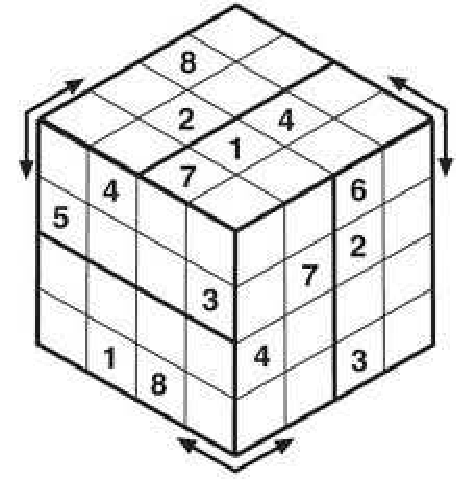
\includegraphics[width=0.3\textwidth]{images}
 \caption{这是一个图片测试例子(中)}
 \label{fig:amss1}
\end{figure}

该页是专门用来测试插入图片的方法,这个方法有很多种,需要自己花点时间来研究学习下,就像表格一样,
下面这只是一个简单的例子。好了,结束。

\subsection{图形位于页面上}
该页是专门用来测试插入图片的方法,这个方法有很多种,需要自己花点时间来研究学习下,就像表格一样,
下面这只是一个简单的例子。好了,结束。该页是专门用来测试插入图片的方法,这个方法有很多种,需要自己花点时间来研究学习下,就像表格一样,
下面这只是一个简单的例子。好了,结束。

\begin{figure}[t]
 \centering
 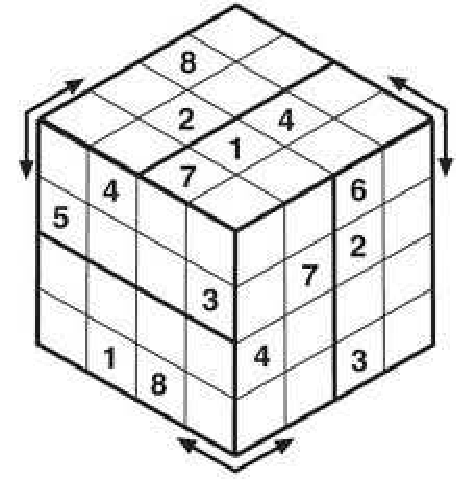
\includegraphics[width=0.3\textwidth]{images}
 \caption{这是一个图片测试例子(上)}
 \label{fig:amss2}
\end{figure}

该页是专门用来测试插入图片的方法,这个方法有很多种,需要自己花点时间来研究学习下,就像表格一样,
下面这只是一个简单的例子。该页是专门用来测试插入图片的方法,这个方法有很多种,需要自己花点时间
来研究学习下,就像表格一样,下面这只是一个简单的例子。该页是专门用来测试插入图片的方法,这个方法
有很多种,需要自己花点时间来研究学习下,就像表格一样,下面这只是一个简单的例子。

\subsection{图形位于页面下}
该页是专门用来测试插入图片的方法,这个方法有很多种,需要自己花点时间来研究学习下,就像表格一样,
下面这只是一个简单的例子。

\begin{figure}[b]
 \centering
 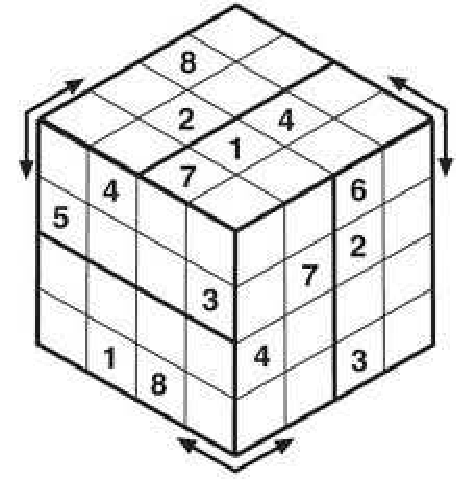
\includegraphics[width=0.3\textwidth]{images}
 \caption{这是一个图片测试例子(下)}
 \label{fig:amss3}
\end{figure}


该页是专门用来测试插入图片的方法,这个方法有很多种,需要自己花点时间来研究学习下,就像表格一样,
下面这只是一个简单的例子。该页是专门用来测试插入图片的方法,这个方法有很多种,需要自己花点时间
来研究学习下,就像表格一样,下面这只是一个简单的例子。

该页是专门用来测试插入图片的方法,这个方法
有很多种,需要自己花点时间来研究学习下,就像表格一样,下面这只是一个简单的例子。该页是专门用来测
试插入图片的方法,这个方法有很多种,需要自己花点时间来研究学习下,就像表格一样,
下面这只是一个简单的例子。

该页是专门用来测试插入图片的方法,这个方法有很多种,需要自己花点时间来研究学习下,就像表格一样,
下面这只是一个简单的例子。该页是专门用来测试插入图片的方法,这个方法有很多种,需要自己花点时间
来研究学习下,就像表格一样,下面这只是一个简单的例子。

该页是专门用来测试插入图片的方法,这个方法
有很多种,需要自己花点时间来研究学习下,就像表格一样,下面这只是一个简单的例子。该页是专门用来测
试插入图片的方法,这个方法有很多种,需要自己花点时间来研究学习下,就像表格一样,
下面这只是一个简单的例子。

该页是专门用来测试插入图片的方法,这个方法有很多种,需要自己花点时间来研究学习下,就像表格一样,
下面这只是一个简单的例子。该页是专门用来测试插入图片的方法,这个方法有很多种,需要自己花点时间
来研究学习下,就像表格一样,下面这只是一个简单的例子。该页是专门用来测试插入图片的方法,这个方法
有很多种,需要自己花点时间来研究学习下,就像表格一样,下面这只是一个简单的例子。该页是专门用来测
试插入图片的方法,这个方法有很多种,需要自己花点时间来研究学习下,就像表格一样,
下面这只是一个简单的例子。

